% Spring Web开发篇
% 
% zzy.hit@gmail.com
% 2013/05/24

\documentclass[xcolor=dvipsnames]{beamer}
\usetheme{Warsaw}
\setbeamertemplate{items}[circle]
\definecolor{links}{HTML}{2A1B81}
\hypersetup{colorlinks,linkcolor=,urlcolor=links}
\usepackage{CJKutf8}
\usepackage{verbatim}

\title{Spring Web Development}
\subtitle{Build web application using jdbc and webmvc}
\author{zzy.hit@gmail.com}
\date{\today}

\begin{document}
\begin{CJK}{UTF8}{gkai}


  % title page 
  \frame{\titlepage}

  \frame{\frametitle{内容}
    \begin{itemize}
      \item Spring Jdbc
      \item Listener, Filter, Servlet
      \item Model-View-Controller
      \item Spring Web
    \end{itemize}
  }

  \frame{\frametitle{目标}
    \begin{itemize}
      \item 理解MVC
      \item 能够使用SpringJdbc及事务
      \item 能够使用Spring构建Web应用
    \end{itemize}
  }

  \frame{\frametitle{Spring Framework}
    \begin{center}
      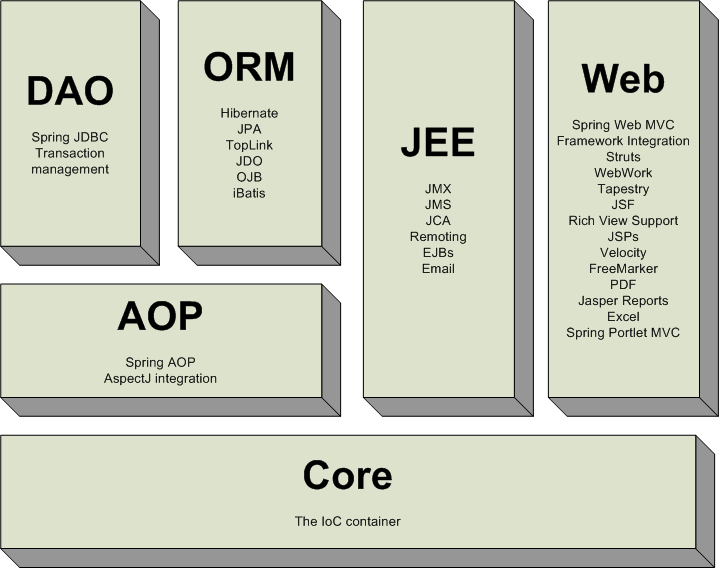
\includegraphics[width=0.9\textwidth]{../spring_framework.png}
    \end{center}
  }

  \frame{\frametitle{Spring Jdbc}
    \begin{center}
      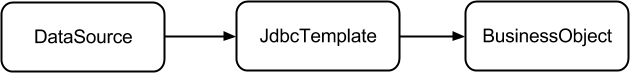
\includegraphics[width=0.8\textwidth]{../jdbctemplate_inject.png}
    \end{center}
    \pause
    \verbatiminput{../jdbc-template.xml}
  }
  \frame{\frametitle{Spring Jdbc}
    常用方法
    \begin{itemize}
      \item query
      \item queryForObject
      \item queryForList
      \item queryForMap
      \item update
      \item batchUpdate
    \end{itemize}
    常用参数
    \begin{itemize}
      \item RowMapper
      \item RowCallbackHandler
      \item BatchPreparedStatementSetter
    \end{itemize}
  }

  \frame{\frametitle{事务}
    \verbatiminput{../transaction.xml}
  }

  \frame{\frametitle{MVC模型}
    \begin{center}
      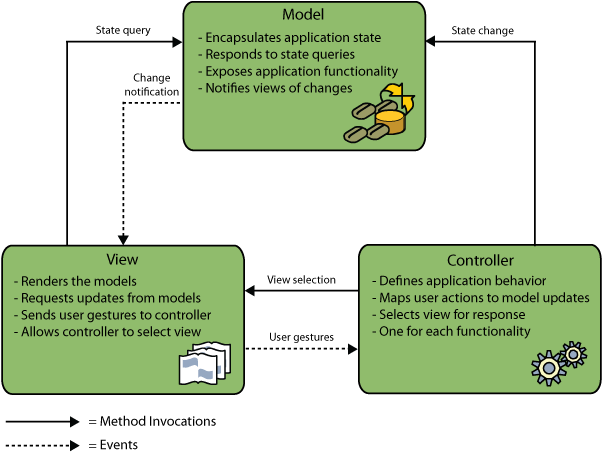
\includegraphics[width=0.9\textwidth]{../mvc-model.png}
    \end{center}
  }

  \frame{\frametitle{Spring MVC 处理过程}
    \begin{center}
      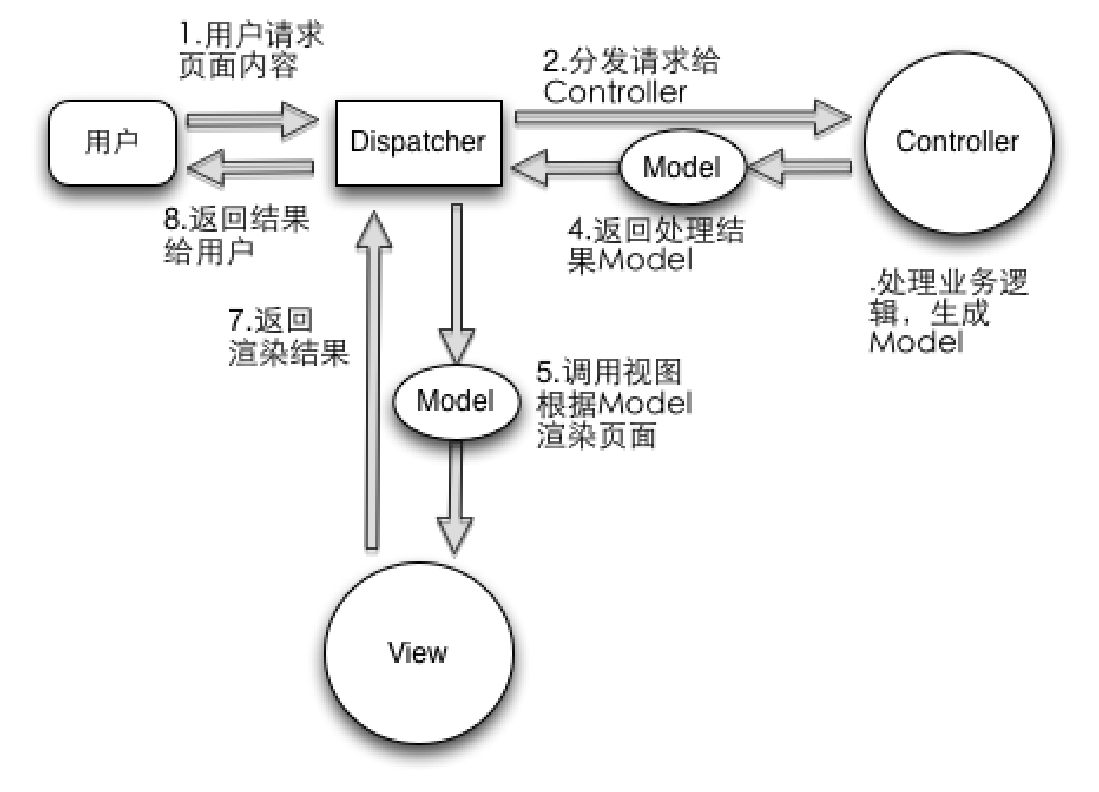
\includegraphics[width=0.85\textwidth]{../spring-mvc.png}
    \end{center}
  }

  \frame{\frametitle{Spring MVC 处理过程}
    \begin{center}
      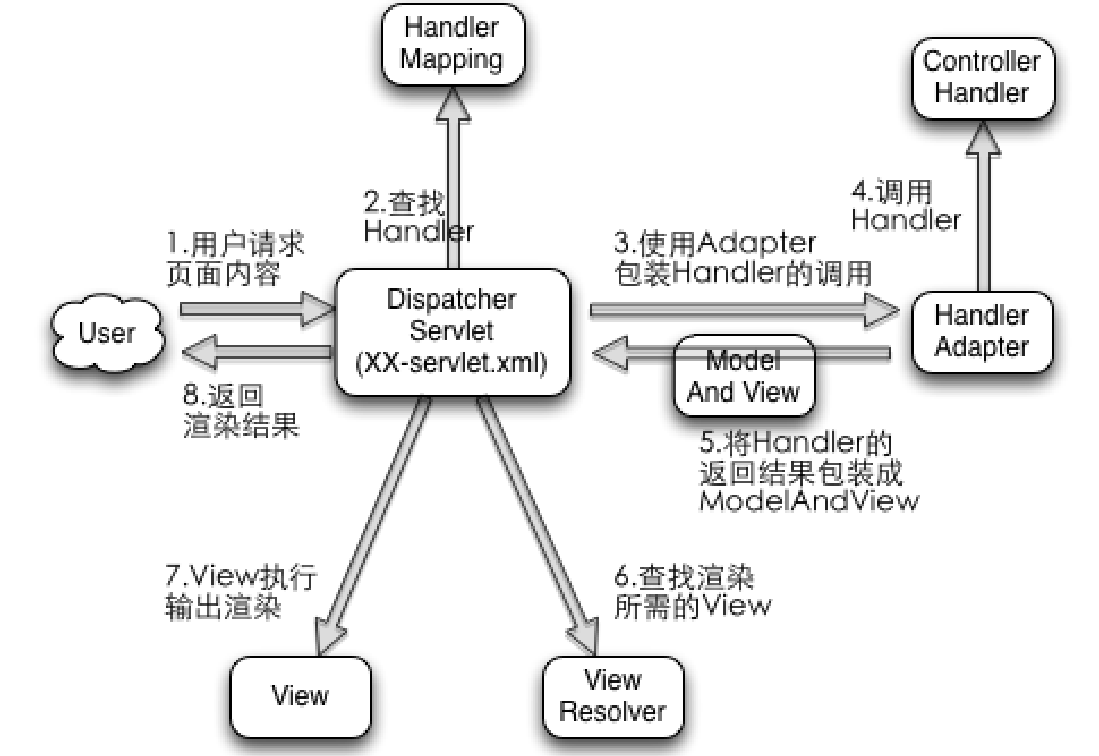
\includegraphics[width=0.85\textwidth]{../spring-workflow.png}
    \end{center}
  }

  \frame{\frametitle{web.xml - ContextLoaderListener}
    \verbatiminput{../context-load-listener.xml}
    \pause
    \begin{itemize}
      \item dao.xml (dataSource, jdbcTemplate, TransactionManager..)
      \item service.xml (service component-scan)
    \end{itemize}
  }

  \frame{\frametitle{web.xml - DispatchServlet}
    \verbatiminput{../dispatcher-servlet.xml}
    \pause
    \begin{itemize}
    \item web-servlet.xml (handler, adapter, resolver, controller)
    \end{itemize}
  }

  \frame{\frametitle{元素}
    \begin{itemize}
    \item WebApplicationContext
    \item HandlerMapping
    \item HandlerAdapter
    \item Controller
    \item ModelAndView
    \item ViewResolver
    \item ExceptionResolver
    \end{itemize}
  }

  \frame{\frametitle{附加了解}
    \begin{itemize}
    \item Validator
    \item Locale, Message
    \item RequestContextHandlingFilter
    \item Quartz
    \end{itemize}
  }

  \frame{\frametitle{MVC常用Annotation}
    \begin{itemize}
    \item @Controller
    \item @RequestMapping
    \item @RequestParam, @PathVariable, @CookieValue
    \item @RequestBody, @ResponseBody
    \end{itemize}
  }

  \frame{\frametitle{ViewResolver}
    返回值
    \begin{itemize}
    \item ModelAndView
    \item String, Object [@ResponseBody]
    \end{itemize}

    常用ViewResolver
    \begin{itemize}
    \item InternalResourceViewResolver
    \item VelocityViewResolver
    \item MappingJacksonJsonView (jackson-core-asl/jackson-mapper-asl)
    \end{itemize}
  }

  \frame{\frametitle{启动过程}
    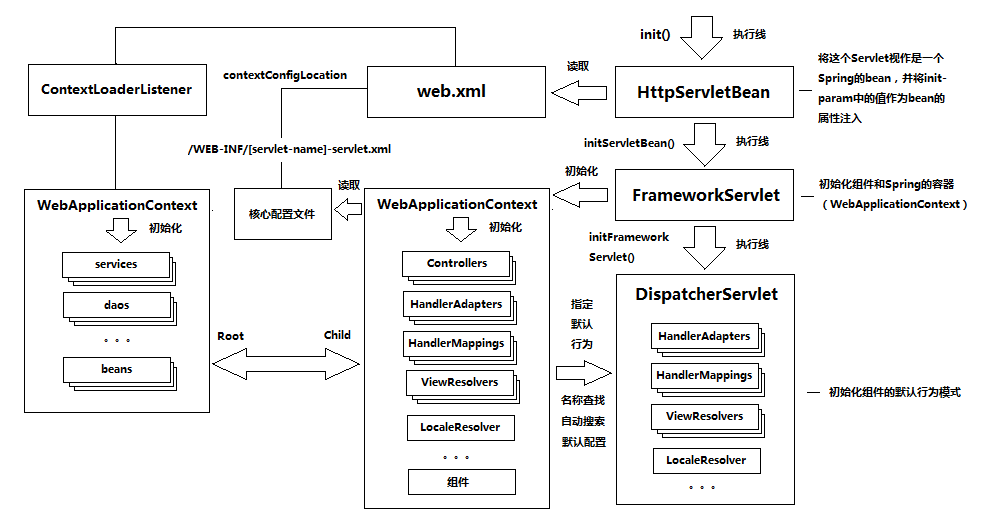
\includegraphics[width=1.1\textwidth]{../spring_init.png}
  }

  \frame{\frametitle{Homework}
    使用Spring实现账户管理,包含列表/查询/添加/更新,要求
    \begin{itemize}
    \item 记录账户变更历史(事务处理)
    \item 添加/更新需登录(Cookie校验)
    \item 列表/查询无需登录

      (控制页面访问可参考RequestContextHandlingFilter实现)
    \end{itemize}
  }

  \frame[plain]{
    \begin{center}
      -EOF-
    \end{center}
  }

\end{CJK}
\end{document}
